\chapter{Stand der Technik}
\label{cha:standdertechnik}
Microsoft Dynamics NAV hat während seiner Entwicklung einige Architektursprünge hingelegt. Ausgehend von Navision für DOS zum Sprung als reine 2-Schichten-Architektur mit FAT-Client zur heutigen 3-Schichten Architektur. \cite{Sah2016}
\begin{figure}[h]
	\centering\small
	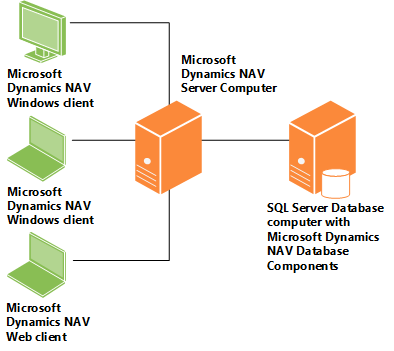
\includegraphics{images/nav_roletailoredarchitecture.png}
	\caption{Overview: Dynamics NAV 3-Tier-Architecture https://docs.microsoft.com/en-us/dynamics-nav/product-and-architecture-overview}
	\label{fig:Image3TierArchitecture}
\end{figure}

Abbildung \ref{fig:Image3TierArchitecture} zeigt einen vereinfachten Grundaufbau der 3-Schichten-Architektur von Dynamics NAV. In Grün sehen wir die verschiedenen Client-Arten die die erste Schicht repräsentieren. Neben dem klassischen Windows-Client zählen auch der Web-Client und die verschiedenen Mobile-Apps zur Schicht Eins. Auf der Schicht Zwei befindet sich der NAV-Server. Dieser bildet den Kern ges Gesamtsystems, verbindet die Datenbank mit den Clients und führt sämtliche Geschäftslogik aus. Die dritte Schicht bildet die Datenbank, auf der sämtliche Datenbestände des Systems verwaltet und persistiert werden. Als Datenbanksystem wird hier Microsoft SQL Server verwendet. 
 Die Serverkomponenten (Server, Datenbank) können sowohl lokal installiert werden, als auch in die Cloud (Microsoft Azure) ausgelagert werden, wobei sämtliche Kombinationen möglich sind, und man daher freie Hand bei der Auswahl der Betriebsoptionen hat.
